% Importado desde: 2026-03-28_Comparacion_Causalidad_Tiempo_Continuo_y_Discreto.tex
\chapter{Derivacion Pedagogica: --- comparacion entre causalidad en tiempo continuo --- y tiempo discreto tipo quantum walk/QCA}
\label{ch:causalidad-continuo-vs-discreto}

\section{Objetivo}
En el capitulo anterior demostramos algo importante: la localidad microscopica induce una velocidad maxima de propagacion y, con ella, una primera nocion de cono causal efectivo.

Ahora toca comparar con cuidado las dos rutas principales del proyecto:
\begin{enumerate}[label=\arabic*.]
    \item \textbf{red espacial discreta y tiempo continuo};
    \item \textbf{espacio-tiempo discreto con evolucion unitaria local tipo quantum walk/QCA}.
\end{enumerate}

La pregunta central sera:
\begin{displayquote}
\textbf{cual de estas dos estrategias ofrece una base mas natural para interpretar la dinamica emergente como proto-espacio-tiempo?}
\end{displayquote}

\section{El punto de comparacion correcto}
No vamos a comparar las dos rutas solo por comodidad algebraica. La comparacion correcta debe hacerse segun cuatro criterios:
\begin{enumerate}[label=\arabic*.]
    \item como se define la dinamica fundamental;
    \item como aparece la causalidad;
    \item que tan fuerte es el cono de propagacion;
    \item que tan natural es la lectura geometrica del tiempo emergente.
\end{enumerate}

\begin{figure}[h!]
\centering
\begin{tikzpicture}[
    box/.style={draw, rounded corners, thick, align=center, minimum width=4cm, minimum height=1.1cm},
    arr/.style={-{Latex[length=3mm]}, thick}
]
\node[box, fill=blue!8] (a) at (0,0) {objeto dinamico\\fundamental};
\node[box, fill=green!8] (b) at (4.8,0) {causalidad\\microscopica};
\node[box, fill=yellow!12] (c) at (9.6,0) {cono de\\propagacion};
\node[box, fill=red!8] (d) at (14.4,0) {lectura de\\proto-espacio-tiempo};
\draw[arr] (a) -- (b);
\draw[arr] (b) -- (c);
\draw[arr] (c) -- (d);
\end{tikzpicture}
\caption{Los cuatro niveles en los que haremos la comparacion.}
\end{figure}

\section{Ruta A: tiempo continuo con Hamiltoniano local}
\subsection{Objeto fundamental}
En esta ruta, el objeto central es un Hamiltoniano local \(H\). La evolucion es
\begin{equation}
i\partial_t \ket{\Psi(t)} = H\ket{\Psi(t)},
\qquad
\ket{\Psi(t)} = e^{-iHt}\ket{\Psi(0)}.
\label{eq:cont-evol}
\end{equation}

La red es discreta, pero el tiempo es un parametro continuo desde el comienzo.

\subsection{Como aparece la causalidad}
Si \(H\) solo conecta vecinos cercanos, entonces:
\begin{enumerate}[label=\arabic*.]
    \item \(H\) mueve la amplitud un numero finito de enlaces por accion;
    \item \(H^r\) solo puede propagar hasta una distancia proporcional a \(r\);
    \item al expandir \(e^{-iHt}\), la amplitud a gran distancia queda muy suprimida para tiempos pequenos.
\end{enumerate}

En el capitulo anterior resumimos esto en una cota del tipo
\begin{equation}
\abs{\mel{\bm{n}}{U(t)}{\bm{m}}}
\lesssim
e^{\norm{H}t}\left(\frac{e\norm{H}t}{L}\right)^L,
\qquad L=d(\bm{n},\bm{m}).
\label{eq:LRped}
\end{equation}

\subsection{Lectura fisica}
La causalidad es aqui \textbf{efectiva}: fuera del cono microscopico la amplitud no es exactamente cero, pero queda fuertemente suprimida.

\begin{figure}[h!]
\centering
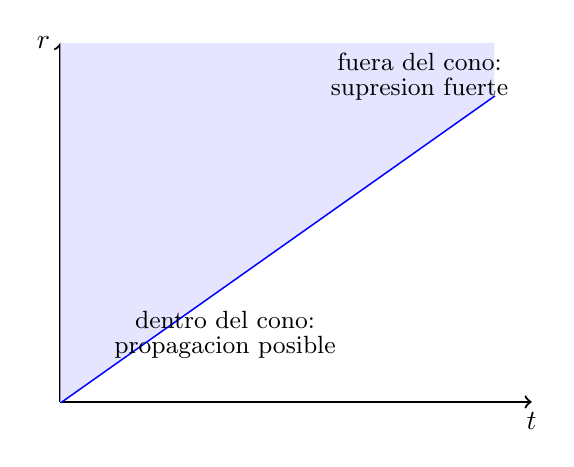
\begin{tikzpicture}[scale=0.95]
\draw[->, thick] (0,0) -- (0,4.8) node[left] {\(r\)};
\draw[->, thick] (0,0) -- (6.3,0) node[below] {\(t\)};
\draw[very thick, blue] (0,0) -- (5.8,4.1);
\fill[blue!10] (0,0) -- (5.8,4.1) -- (5.8,4.8) -- (0,4.8) -- cycle;
\node[align=center] at (2.2,0.9) {\small dentro del cono:\\[-1mm]\small propagacion posible};
\node[align=center] at (4.8,4.35) {\small fuera del cono:\\[-1mm]\small supresion fuerte};
\end{tikzpicture}
\caption{En tiempo continuo la localidad genera un cono efectivo con colas suprimidas, no un soporte exactamente compacto.}
\end{figure}

\subsection{Ventaja conceptual}
Esta ruta conecta de forma muy natural con:
\begin{enumerate}[label=\arabic*.]
    \item SSH;
    \item grafeno;
    \item semimetales de Dirac y Weyl;
    \item Hamiltonianos de Wilson.
\end{enumerate}

Es la ruta mas cercana a la intuicion de materia condensada y a la construccion por linealizacion de bandas.

\subsection{Limitacion conceptual}
El tiempo no se construye: ya esta dado desde el inicio. Por eso, si la meta es un \enquote{espacio-tiempo emergente}, esta estrategia tiene un limite claro:
\begin{displayquote}
\textbf{permite estudiar muy bien el espacio discreto y la relatividad efectiva, pero no reconstruye el tiempo como parte de la microestructura.}
\end{displayquote}

\section{Ruta B: tiempo discreto con quantum walk o QCA}
\subsection{Objeto fundamental}
En esta ruta el objeto central no es un Hamiltoniano, sino un operador unitario local \(U\):
\begin{equation}
\ket{\Psi_{n+1}} = U\ket{\Psi_n}.
\label{eq:disc-evol}
\end{equation}

Aqui \(n\) cuenta pasos temporales separados por \(\Delta t\). El tiempo ya no es primitivo y continuo, sino que tambien aparece discretizado.

\subsection{Como aparece la causalidad}
Si en un solo paso la amplitud puede desplazarse, como mucho, una distancia \(a\), entonces:
\begin{enumerate}[label=\arabic*.]
    \item despues de un paso solo hay soporte en la primera vecindad;
    \item despues de dos pasos solo en la segunda;
    \item despues de \(N\) pasos solo dentro de una region de radio proporcional a \(Na\).
\end{enumerate}

\subsection{Demostracion elemental}
Sea \(S_N\) el soporte del estado tras \(N\) pasos.

\subsubsection*{Paso inicial}
Si el estado empieza localizado en \(\bm{x}_0\), entonces
\begin{equation}
S_0 = \{\bm{x}_0\}.
\end{equation}

\subsubsection*{Un paso}
Como \(U\) es local, tras un paso el soporte solo puede ocupar los sitios vecinos permitidos por la regla elemental:
\begin{equation}
S_1 \subseteq B_1(\bm{x}_0),
\end{equation}
donde \(B_1\) es la bola de radio un paso.

\subsubsection*{Paso inductivo}
Si tras \(N\) pasos vale
\begin{equation}
S_N \subseteq B_N(\bm{x}_0),
\end{equation}
entonces al aplicar un paso mas:
\begin{equation}
S_{N+1} \subseteq B_{N+1}(\bm{x}_0).
\end{equation}

Por induccion:
\begin{equation}
S_N \subseteq B_N(\bm{x}_0).
\label{eq:exactsupport}
\end{equation}

\subsection{Lectura fisica}
La causalidad es aqui \textbf{exacta a nivel microscópico}. Fuera del cono permitido por la regla local:
\begin{equation}
\text{soporte} = 0.
\end{equation}

\begin{figure}[h!]
\centering
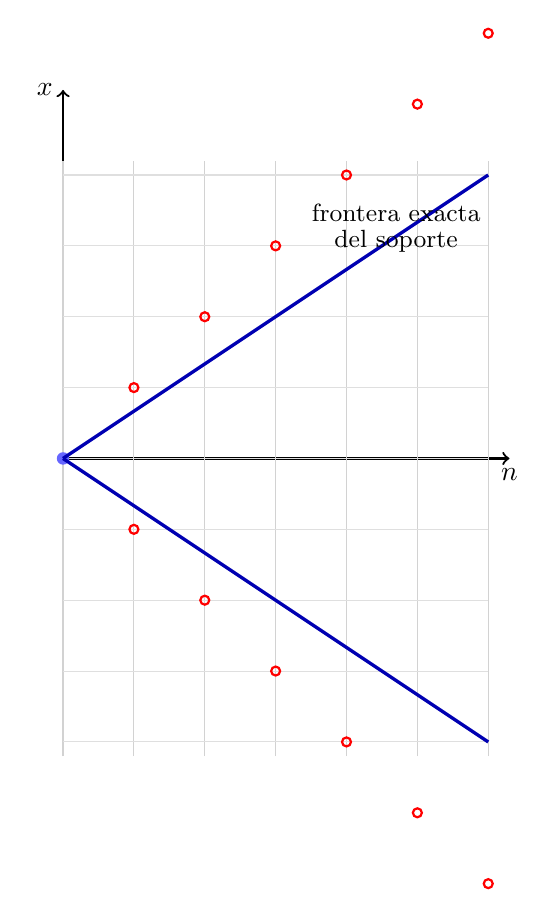
\begin{tikzpicture}[scale=0.9]
\draw[->, thick] (0,0) -- (0,5.2) node[left] {\(x\)};
\draw[->, thick] (0,0) -- (6.3,0) node[below] {\(n\)};
\foreach \n in {0,1,2,3,4,5,6}{
    \draw[gray!35] (\n,-4.2) -- (\n,4.2);
}
\foreach \x in {-4,-3,-2,-1,0,1,2,3,4}{
    \draw[gray!25] (0,\x) -- (6,\x);
}
\fill[blue!60] (0,0) circle (2.5pt);
\foreach \n/\m in {1/1,2/2,3/3,4/4,5/5,6/6}{
    \draw[thick, red] (\n,\m) circle (1.8pt);
    \draw[thick, red] (\n,-\m) circle (1.8pt);
}
\draw[very thick, blue!70!black] (0,0) -- (6,4);
\draw[very thick, blue!70!black] (0,0) -- (6,-4);
\node[align=center] at (4.7,3.25) {\small frontera exacta\\[-1mm]\small del soporte};
\end{tikzpicture}
\caption{En tiempo discreto local, el cono causal puede ser exacto: fuera de el no hay soporte.}
\end{figure}

\subsection{Velocidad microscopica}
Si cada paso dura \(\Delta t\), entonces:
\begin{equation}
r \le Na = \frac{a}{\Delta t} t.
\end{equation}

La velocidad maxima elemental es
\begin{equation}
c_\ast = \frac{a}{\Delta t}.
\label{eq:cstar}
\end{equation}

Aqui la velocidad limite no sale de una cota asintotica, sino de la propia definicion de la dinamica.

\section{Como emerge Dirac en cada ruta}
\subsection{En tiempo continuo}
En la ruta Hamiltoniana, Dirac emerge por linealizacion de \(H(\bm{k})\) cerca de un nodo:
\begin{equation}
H(\bm{k}_0+\bm{q}) \simeq v\sum_i q_i \alpha_i + m\beta.
\label{eq:dirac-cont}
\end{equation}

La velocidad \(v\) aparece como pendiente del cono de Dirac. Debe ser compatible con la velocidad microscopica inducida por la localidad.

\subsection{En tiempo discreto}
En una caminata cuantica minima, el paso puede escribirse simbolicamente como
\begin{equation}
U(\bm{k}) \simeq \mathbb{I} - i\Delta t\,H_{\text{eff}}(\bm{k}),
\end{equation}
de donde se extrae un Hamiltoniano efectivo:
\begin{equation}
H_{\text{eff}}(\bm{k}) \simeq v\sum_i q_i \alpha_i + m\beta.
\label{eq:dirac-disc}
\end{equation}

La diferencia crucial es que ahora:
\begin{enumerate}[label=\arabic*.]
    \item el tiempo continuo efectivo sale de una expansion de la dinamica por pasos;
    \item la velocidad \(v\) queda anclada a la escala elemental \(a/\Delta t\).
\end{enumerate}

\subsection{Ejemplo pedagogico en 1D}
Si un paso elemental tiene la forma aproximada
\begin{equation}
U(k)\simeq \mathbb{I} - i\left(ak\,\sigma_z + \theta \sigma_y\right),
\end{equation}
entonces, identificando \(U \simeq \mathbb{I} - i\Delta t H_{\text{eff}}\), obtenemos
\begin{equation}
H_{\text{eff}}(k)
\simeq
\frac{a}{\Delta t}k\,\sigma_z
+ \frac{\theta}{\Delta t}\sigma_y.
\label{eq:qw-dirac}
\end{equation}

Vemos inmediatamente que:
\begin{equation}
v = \frac{a}{\Delta t},
\qquad
m = \frac{\theta}{\Delta t}.
\end{equation}

Esta identificacion es muy valiosa: la velocidad del continuo efectivo coincide naturalmente con la velocidad elemental de propagacion del modelo por pasos.

\section{La diferencia central}
Con todo esto, la diferencia mas profunda puede formularse asi:

\subsection{Tiempo continuo}
\begin{enumerate}[label=\arabic*.]
    \item la causalidad aparece a partir de la localidad de \(H\);
    \item el cono es efectivo y viene con colas suprimidas;
    \item el tiempo no emerge: ya estaba dado.
\end{enumerate}

\subsection{Tiempo discreto}
\begin{enumerate}[label=\arabic*.]
    \item la causalidad esta codificada directamente en la regla de actualizacion;
    \item el cono puede ser exacto a nivel microscopico;
    \item el tiempo efectivo continuo emerge a partir de pasos discretos.
\end{enumerate}

\begin{figure}[h!]
\centering
\begin{tikzpicture}[
    box/.style={draw, rounded corners, thick, align=left, text width=5.4cm, inner sep=6pt},
    arr/.style={-{Latex[length=3mm]}, thick}
]
\node[box, fill=blue!8] (a) at (0,0) {Tiempo continuo\\[1mm]
\(H\) local \(\to e^{-iHt}\)\\
cono efectivo\\
tiempo dado desde el inicio};
\node[box, fill=green!8] (b) at (8.5,0) {Tiempo discreto\\[1mm]
\(U\) local por pasos\\
cono exacto o cuasi-exacto\\
tiempo continuo como limite};
\draw[arr] (a.east) -- node[above] {\small comparacion estructural} (b.west);
\end{tikzpicture}
\caption{La diferencia clave no es solo tecnica, sino conceptual.}
\end{figure}

\section{Que ruta favorece mejor la idea de proto-espacio-tiempo}
Si el objetivo fuera solo obtener Dirac efectivo, las dos rutas son validas.

Pero si afinamos la pregunta y pedimos:
\begin{displayquote}
\textbf{que construccion ofrece una base mas natural para que tambien el tiempo y la causalidad formen parte de la microestructura?}
\end{displayquote}

entonces la ruta de tiempo discreto parece mas prometedora.

\subsection{Por que}
\begin{enumerate}[label=\arabic*.]
    \item porque la causalidad elemental no se deduce despues, sino que esta incorporada desde el principio;
    \item porque el tiempo no se presupone continuo;
    \item porque la velocidad limite sale de la propia regla local;
    \item porque la reconstruccion del continuo efectivo se parece mas a una emergencia genuina de espacio-tiempo.
\end{enumerate}

\subsection{Pero sin exagerar}
Esto no significa que el problema este resuelto. Aun en tiempo discreto quedan cuestiones delicadas:
\begin{enumerate}[label=\arabic*.]
    \item como obtener isotropia suficientemente buena en varias dimensiones;
    \item como controlar duplicacion fermionica y sectores no deseados;
    \item como conectar la simetria efectiva con la estructura de Lorentz y sus representaciones espinoriales.
\end{enumerate}

\section{Una tabla comparativa}
\begin{center}
\begin{tabular}{p{4.3cm} p{5.2cm} p{5.2cm}}
\toprule
Aspecto & Tiempo continuo & Tiempo discreto tipo QW/QCA \\
\midrule
Objeto fundamental & Hamiltoniano \(H\) & operador unitario \(U\) \\
Causalidad microscopica & efectiva, tipo Lieb--Robinson & exacta o cuasi-exacta por paso local \\
Velocidad maxima & surge de una cota & viene de \(a/\Delta t\) \\
Estado del tiempo & continuo desde el inicio & discreto en la base \\
Emergencia de Dirac & linealizacion de \(H(\bm{k})\) & expansion de \(U(\bm{k})\) \\
Ventaja principal & conexion directa con bandas y materiales & mejor punto de apoyo para proto-espacio-tiempo \\
Dificultad principal & el tiempo no emerge & isotropia y simetrias en dimensiones altas \\
\bottomrule
\end{tabular}
\end{center}

\section{Que conclusion metodologica debemos sacar}
La comparacion no nos obliga a abandonar la ruta Hamiltoniana. Al contrario: esa ruta sigue siendo indispensable para construir intuicion, estudiar nodos, entender subredes, quiralidad y estructura Clifford.

Pero si no queremos perder de vista la meta final del proyecto, la conclusion metodologica es esta:
\begin{displayquote}
\textbf{la ruta Hamiltoniana es la mejor escuela para construir el contenido efectivo de Dirac; la ruta de tiempo discreto es la candidata mas seria para convertir ese contenido en una microdinamica con lectura de proto-espacio-tiempo.}
\end{displayquote}

\section{Mapa del siguiente paso}
El siguiente paso natural, siguiendo exactamente esta conclusion, es:
\begin{enumerate}[label=\arabic*.]
    \item tomar una construccion concreta de quantum walk/QCA;
    \item analizar con detalle su isotropia y su estructura de simetrias;
    \item ver en que medida reproduce no solo Dirac, sino tambien una causalidad y una geometria efectivas suficientemente limpias.
\end{enumerate}

\begin{figure}[h!]
\centering
\begin{tikzpicture}[
    box/.style={draw, rounded corners, thick, align=center, minimum width=4cm, minimum height=1.1cm},
    arr/.style={-{Latex[length=3mm]}, thick}
]
\node[box, fill=blue!7] (a) at (0,0) {causalidad efectiva\\en tiempo continuo};
\node[box, fill=green!7] (b) at (5,0) {comparacion\\con tiempo discreto};
\node[box, fill=yellow!12] (c) at (10,0) {QW/QCA concreto\\con simetrias};
\node[box, fill=red!7] (d) at (15,0) {proto-geometria\\mas solida};
\draw[arr] (a) -- (b);
\draw[arr] (b) -- (c);
\draw[arr] (c) -- (d);
\end{tikzpicture}
\caption{La comparacion de este capitulo abre el camino hacia una construccion discreta mas completa.}
\end{figure}

\section{Resumen final}
Las dos rutas del proyecto producen fermiones de Dirac efectivos, pero no lo hacen desde el mismo punto conceptual. En tiempo continuo, la causalidad surge como consecuencia de la localidad del Hamiltoniano y el cono de propagacion es efectivo, con colas suprimidas. En tiempo discreto, la causalidad viene codificada desde el comienzo en la regla local de evolucion, y el cono puede ser exacto a nivel microscopico.

Por eso, si la meta inmediata es entender bien la fisica efectiva, la ruta Hamiltoniana sigue siendo insustituible. Pero si la meta de fondo es investigar una posible lectura de espacio-tiempo emergente, la ruta de tiempo discreto tipo quantum walk/QCA parece mas prometedora. No porque ya resuelva todo, sino porque trata a la causalidad y al tiempo como parte de la propia microestructura, y no como ingredientes heredados desde afuera.
